\documentclass[12pt, twoside]{article}
\usepackage[letterpaper, margin=1in, headsep=0.5in]{geometry}
\usepackage[english]{babel}
\usepackage[utf8]{inputenc}
\usepackage{amsmath}
\usepackage{amsfonts}
\usepackage{amssymb}
\usepackage{tikz}
\usepackage{yhmath}
%\usetikzlibrary{quotes, angles}

\usepackage{graphicx}
\usepackage{enumitem}
\usepackage{multicol}

\usepackage{fancyhdr}
\pagestyle{fancy}
\fancyhf{}
\renewcommand{\headrulewidth}{0pt} % disable the underline of the header

\fancyhead[RE]{\thepage}
\fancyhead[RO]{\thepage \\ Name: \hspace{3cm}}
\fancyhead[L]{BECA / Dr. Huson / 10th Grade Geometry\\* 1 April 2019}

\begin{document}
\subsubsection*{9.5 Do Now: Angle relationships}
 \begin{enumerate}

\item The figure shows a rectangle (not a square).
  \begin{center}
    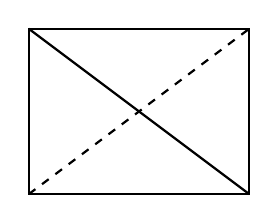
\begin{tikzpicture}[scale=0.7]
      \coordinate (A) at (0, 0); %[label=above left:$P$]
      \coordinate (B) at (4, 0);
      \coordinate (C) at (4, 3);
      \coordinate (D) at (0, 3);
      \draw [thick] (A)--(B)--(C)--(D)--cycle;
      \draw [thick, dashed] (A)--(C);
      \draw [thick] (B)--(D);
      %\draw [thick, xshift=2cm, yshift=2.5cm] (85:3);
    \end{tikzpicture}
  \end{center}
  Which transformations carries the rectangle onto itself? Mark each True or False.
    \begin{enumerate}
      \item A clockwise rotation of $90^\circ$ about the intersection of the diagonals \hfill True \quad False
      \item A clockwise rotation of $180^\circ$ about the intersection of the diagonals \hfill True \quad False
      \item A reflection over the solid diagonal \hfill True \quad False
      \item A reflection over the dashed diagonal \hfill True \quad False
    \end{enumerate}

       \item Find the area of $\triangle ABC$,  $Area= \frac{1}{2}bh$. The altitude $h$ of the triangle is 4 centimeters and the base $AB=7.3$ cm.\\[1cm]
       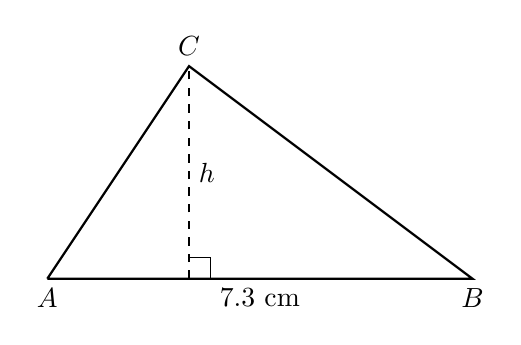
\begin{tikzpicture}[scale=0.9]
         \draw [thick]
           (2,0)node[below]{$A$}--
           (8,0)node[below]{$B$}--
           (4,3)node[above]{$C$} --(2,0);
        \draw [dashed] (4,0)--(4,3);
        \draw (4,0)++(0.3,0)--++(0,0.3)--+(-0.3,0);
        \node at (4,1.5)[right]{$h$};
        \node at (5,0)[below]{$7.3$ cm};
       \end{tikzpicture}

   \item Given  $\triangle EFG$ with $m\angle E=(10x)^\circ$, $m\angle F=40^\circ$ and $m\angle G=(6x+60)^\circ$, find $x$.
     \begin{center}
       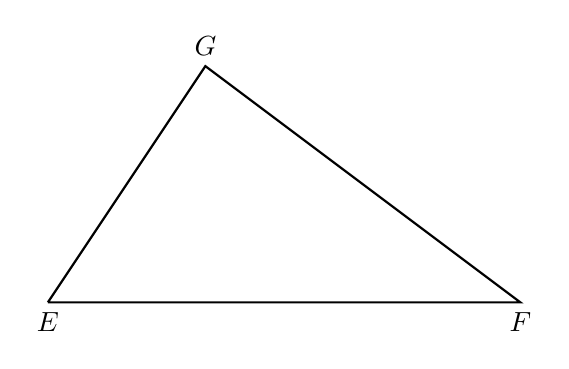
\begin{tikzpicture}%[scale=0.7]
         \draw [thick] %(0,0)node[below]{$A$}--
           (2,0)node[below]{$E$}--
           (8,0)node[below]{$F$}--
           (4,3)node[above]{$G$} --(2,0);
       \end{tikzpicture}
     \end{center} \vspace{3cm}

\newpage


  \item In the diagram below, the chords $\overline{AE}$ and $\overline{BD}$ intersect at $C$, with $m \angle ACB = 5x-5$, $m \angle DCE = 4x+11$.
  \begin{enumerate}
    \item Justify $\angle ACB \cong \angle DCE$. \vspace{1cm}
    \item Find $x$.  \vspace{3cm}
    \item Given that $m \wideparen{AFD}=140^\circ$. Find $m\angle E$. Find $m\angle B$.  \vspace{1cm}
    \item Find $m\angle D$.  \vspace{3cm}
    \item Find the measure of $\wideparen{BE}$.  \vspace{1cm} %note yhmath package
%    \item $\stackrel{\frown}{BE}$

  \end{enumerate}
      \begin{center}
      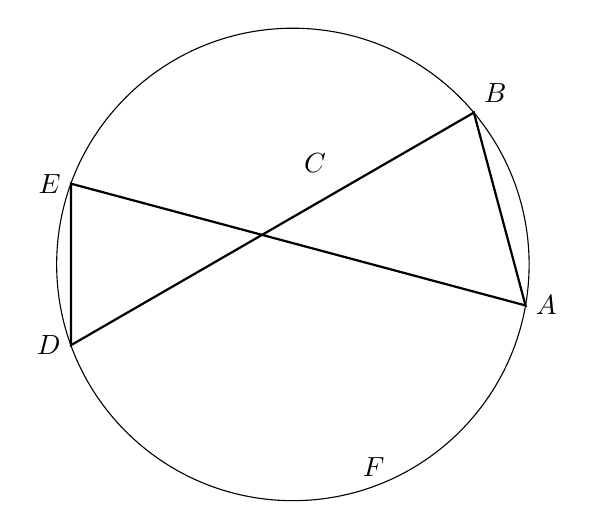
\begin{tikzpicture}[scale=.6]
        \draw (0,0) circle[radius=5];
        \draw [thick]
        (-10:5) node[right] {$A$}--
        (160:5) node[left] {$E$}--
        (200:5) node[left] {$D$}--
        (40:5) node[above right] {$B$}--cycle;
        \draw (75:1.8) node[above] {$C$};
        \draw (290:5) node[above] {$F$};
      \end{tikzpicture}
    \end{center}

\end{enumerate}
\end{document}
